\documentclass[xetex]{beamer}
\usepackage{kotex}
\usetheme{Copenhagen}
\usepackage{fontspec}
\usepackage{xunicode}
\usepackage{xltxtra}
\usefonttheme{serif}
\setmainfont{NanumGothicBold}
\begin{document}
\title{2017 서울대학교 프로그래밍 경시대회}
\date{\today} 

\frame{\titlepage} 

\begin{frame}
  \frametitle{수고하셨습니다}
  \begin{itemize}
    \item 총 참가자 45명
    \item 총 제출 횟수: 931
    \item 총 정답 횟수: 182
    \item 참고로 문제 배치는 랜덤입니다.
  \end{itemize}
\end{frame}

\begin{frame}
  \frametitle{D2-A. 여우 사인}
  \begin{itemize}
    \item 제출 횟수: ??
    \item 맞은 참가자 수: ??
    \item 정답률: ??\%
    \item 처음 맞은 참가자: ??
    \item 출제자: 임동재
  \end{itemize}
\end{frame}

\begin{frame}
  \frametitle{D2-A. 여우 사인}
  \begin{itemize}
    \item 잘 계산하면 돼요.
    \item 단순히 반복문 돌려도 아마 될 거예요.
  \end{itemize}
\end{frame}

\begin{frame}
  \frametitle{D2-B. 고장난 시계}
  \begin{itemize}
    \item 제출 횟수: ??
    \item 맞은 참가자 수: ??
    \item 정답률: ??\%
    \item 처음 맞은 참가자: ??
    \item 출제자: 박상언
  \end{itemize}
\end{frame}

\begin{frame}
  \frametitle{D2-B. 고장난 시계}
  \begin{itemize}
    \item 판이 크지는 않아요.
    \item 반드시 전구가 배치되어야 하는 곳과 그렇지 않은 곳이 있어요.
    \item 나머지는 잘 채워나가면 돼요.
  \end{itemize}
\end{frame}

\begin{frame}
  \frametitle{D2-C. 타일 뒤집기 (Easy)}
  \begin{itemize}
    \item 제출 횟수: ??
    \item 맞은 참가자 수: ??
    \item 정답률: ??\%
    \item 처음 맞은 참가자: ??
    \item 출제자: 임동재
  \end{itemize}
\end{frame}

\begin{frame}
  \frametitle{D2-C. 타일 뒤집기 (Easy)}
  \begin{itemize}
    \item DP!
    \item $k$번째로 XXX 공항에 도착하는 확률을 계산해요.
    \item XXX 공항에 도착하는 코스 중 최대확률의 정보만 저장하면 돼요.
    \item 근데 double 자료형은 생각보다 정확하지 않아요.
    \item 확률의 log값을 저장하도록 하면 해결할 수 있어요.
  \end{itemize}
\end{frame}

\begin{frame}
  \frametitle{D2-D, D1-B. 관악산 등산}
  \begin{itemize}
    \item 제출 횟수: ??
    \item 맞은 참가자 수: ??
    \item 정답률: ??\%
    \item 처음 맞은 참가자: ??
    \item 출제자: 임동재
  \end{itemize}
\end{frame}

\begin{frame}
  \frametitle{D2-D, D1-B. 관악산 등산}
  \begin{columns}
    \column{0.5\textwidth}
      \begin{itemize}
        \item 즐거운 수학 시간
        \item 내접원의 반지름을 구해요.
        \item 현재 원의 반지름이 $r$일 때 다음 원의 반지름을 구할 수 있어요.
      \end{itemize}
    \column{0.5\textwidth}
      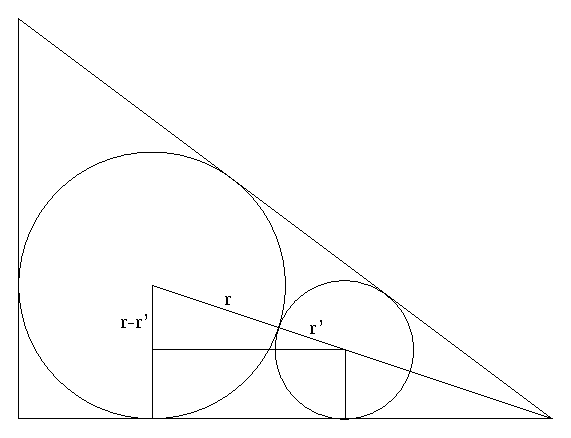
\includegraphics[width=0.9\textwidth]{pizza-solution.eps}
  \end{columns}
\end{frame}

\begin{frame}
  \frametitle{D2-E. 넴모넴모 (Easy)}
  \begin{itemize}
    \item 제출 횟수: ??
    \item 맞은 참가자 수: ??
    \item 정답률: ??\%
    \item 처음 맞은 참가자: ??
    \item 출제자: 임동재
  \end{itemize}
\end{frame}

\begin{frame}
  \frametitle{D2-E. 넴모넴모 (Easy)}
  \begin{itemize}
    \item 세그먼트 트리를 써요.
    \item 각 노드에는 왕의 이름 (및 substring)을 읽는 경우의 수를 2차원 배열로 저장해요.
    \item 그러면 두 노드를 합치는 연산은 $O(m^{3})$이 걸려요.
    \item 전체 시간복잡도는 $O(Pm^{3}\log n)$ ($P = \Sigma|S|$)
    \item 이러면 아마 TLE일걸요?
  \end{itemize}
\end{frame}

\begin{frame}
  \frametitle{D2-F. 앵무새}
  \begin{itemize}
    \item 제출 횟수: ??
    \item 맞은 참가자 수: ??
    \item 정답률: ??\%
    \item 처음 맞은 참가자: ??
    \item 출제자: 오평석
  \end{itemize}
\end{frame}

\begin{frame}
  \frametitle{D2-F. 앵무새}
  \begin{itemize}
    \item 답은 $100,000$ 이하로 나와요.
    \item 모든 가능한 분모에 대해 분자를 구하고, 그 결과가 입력과 같은지를 확인하면 돼요.
  \end{itemize}
\end{frame}

\begin{frame}
  \frametitle{D2-G, D1-D. 셔틀버스}
  \begin{itemize}
    \item 제출 횟수: ??
    \item 맞은 참가자 수: ??
    \item 정답률: ??\%
    \item 처음 맞은 참가자: ??
    \item 출제자: 임동재
  \end{itemize}
\end{frame}

\begin{frame}
  \frametitle{D2-G, D1-D. 셔틀버스}
  \begin{itemize}
    \item 입력에 대해 Suffix Array를 만들어요.
    \item 특정 길이 이상의 원소 중 가장 마지막 원소를 가져와요.
    \item LCP를 찾으면 몇 번 반복됐는지 알 수 있어요.
  \end{itemize}
\end{frame}

\begin{frame}
  \frametitle{D2-H. 홍삼 게임 (Easy)}
  \begin{itemize}
    \item 제출 횟수: ??
    \item 맞은 참가자 수: ??
    \item 정답률: ??\%
    \item 처음 맞은 참가자: ??
    \item 출제자: 임동재
  \end{itemize}
\end{frame}

\begin{frame}
  \frametitle{D2-H. 홍삼 게임 (Easy)}
  \begin{itemize}
    \item 결국 모든 수의 최소공배수를 구하면 답이 돼요.
    \item 모든 수를 소인수분해한 다음, 각 소수마다 지수값의 최대를 취하면 최소공배수를 구할 수 있어요.
  \end{itemize}
\end{frame}

\begin{frame}
  \frametitle{D2-I. 전생했더니 슬라임 연구자였던 건에 대하여 (Easy)}
  \begin{itemize}
    \item 제출 횟수: ??
    \item 맞은 참가자 수: ??
    \item 정답률: ??\%
    \item 처음 맞은 참가자: ??
    \item 출제자: 박성원
  \end{itemize}
\end{frame}

\begin{frame}
  \frametitle{D2-I. 전생했더니 슬라임 연구자였던 건에 대하여 (Easy)}
  \begin{columns}
    \column{0.5\textwidth}
      \begin{itemize}
        \item 결국 오른쪽 영역의 넓이를 구하면 돼요.
        \item 입력된 세 점의 방향에 따라 넓이를 구하는 영역이 달라져요. (회색 또는 노란색)
      \end{itemize}
    \column{0.5\textwidth}
      \includegraphics[width=0.9\textwidth]{torres-solution.eps}
  \end{columns}
\end{frame}

\begin{frame}
  \frametitle{D1-A. 전생했더니 슬라임 연구자였던 건에 대하여 (Hard)}
  \begin{itemize}
    \item 제출 횟수: ??
    \item 맞은 참가자 수: ??
    \item 정답률: ??\%
    \item 처음 맞은 참가자: ??
    \item 출제자: 박성원
  \end{itemize}
\end{frame}

\begin{frame}
  \frametitle{D1-A. 전생했더니 슬라임 연구자였던 건에 대하여 (Hard)}
  \begin{itemize}
    \item offline 풀이 입니다.
    \item 두 승현이의 위치를 나타내는 상태 $(u, v)$를 정점으로 하는 그래프를 생각해요.
    \item 비용이 적은 순서대로 정점을 추가하면서 연결된 컴포넌트들을 유지해요.
    \item $(x, y)$와 $(y, x)$가 연결되는 순간에 추가된 정점의 비용이 $(x, y)$ 의 답이 돼요.
    \item 컴포넌트들은 disjoint-set 으로 관리하면 돼요.
    \item $O(n m + n^{2} log{n})$
  \end{itemize}
\end{frame}

\begin{frame}
  \frametitle{D1-C. 넴모넴모 (Hard)}
  \begin{itemize}
    \item 제출 횟수: ??
    \item 맞은 참가자 수: ??
    \item 정답률: ??\%
    \item 처음 맞은 참가자: ??
    \item 출제자: 임동재
  \end{itemize}
\end{frame}

\begin{frame}
  \frametitle{D1-C. 넴모넴모 (Hard)}
  \begin{itemize}
    \item 가중치의 합이 최소가 되도록 $K+1$개의 트리로 나누는 문제예요.
    \item 모든 트리를 특정 값 이하로 만들 수 있는지를 반복하면 답을 구할 수 있어요. (parametric search)
  \end{itemize}
\end{frame}

\begin{frame}
  \frametitle{D1-E. 데굴데굴}
  \begin{itemize}
    \item 제출 횟수: ??
    \item 맞은 참가자 수: ??
    \item 정답률: ??\%
    \item 처음 맞은 참가자: ??
    \item 출제자: 임동재
  \end{itemize}
\end{frame}

\begin{frame}
  \frametitle{D1-E. 데굴데굴}
  \begin{itemize}
    \item 문제를 풀기 위해 아래 지식이 필요해요.
    \begin{itemize}
      \item 2차원에서 직사각형 영역의 부분합을 빠르게 구하는 방법 (cf. BOJ 11660)
      \item 주어진 히스토그램에서 가장 큰 직사각형의 넓이를 구하는 방법 (cf. BOJ 1725)
      \item 포함배제의 원리
    \end{itemize}
  \end{itemize}
\end{frame}

\begin{frame}
  \frametitle{D1-F. 전자기기}
  \begin{itemize}
    \item 제출 횟수: ??
    \item 맞은 참가자 수: ??
    \item 정답률: ??\%
    \item 처음 맞은 참가자: ??
    \item 출제자: 윤지학
  \end{itemize}
\end{frame}

\begin{frame}
  \frametitle{D1-F. 전자기기}
  \begin{itemize}
    \item 문제를 풀기 위해 아래 지식이 필요해요.
    \begin{itemize}
      \item 2차원에서 직사각형 영역의 부분합을 빠르게 구하는 방법 (cf. BOJ 11660)
      \item 주어진 히스토그램에서 가장 큰 직사각형의 넓이를 구하는 방법 (cf. BOJ 1725)
      \item 포함배제의 원리
    \end{itemize}
  \end{itemize}
\end{frame}

\begin{frame}
  \frametitle{D1-G. 타일 뒤집기 (Hard)}
  \begin{itemize}
    \item 제출 횟수: ??
    \item 맞은 참가자 수: ??
    \item 정답률: ??\%
    \item 처음 맞은 참가자: ??
    \item 출제자: 임동재
  \end{itemize}
\end{frame}

\begin{frame}
  \frametitle{D1-G. 타일 뒤집기 (Hard)}
  \begin{itemize}
    \item 문제를 풀기 위해 아래 지식이 필요해요.
    \begin{itemize}
      \item 2차원에서 직사각형 영역의 부분합을 빠르게 구하는 방법 (cf. BOJ 11660)
      \item 주어진 히스토그램에서 가장 큰 직사각형의 넓이를 구하는 방법 (cf. BOJ 1725)
      \item 포함배제의 원리
    \end{itemize}
  \end{itemize}
\end{frame}

\begin{frame}
  \frametitle{D1-H. 홍삼 게임 (Hard)}
  \begin{itemize}
    \item 제출 횟수: ??
    \item 맞은 참가자 수: ??
    \item 정답률: ??\%
    \item 처음 맞은 참가자: ??
    \item 출제자: 임동재
  \end{itemize}
\end{frame}

\begin{frame}
  \frametitle{D1-H. 홍삼 게임 (Hard)}
  \begin{itemize}
    \item 문제를 풀기 위해 아래 지식이 필요해요.
    \begin{itemize}
      \item 2차원에서 직사각형 영역의 부분합을 빠르게 구하는 방법 (cf. BOJ 11660)
      \item 주어진 히스토그램에서 가장 큰 직사각형의 넓이를 구하는 방법 (cf. BOJ 1725)
      \item 포함배제의 원리
    \end{itemize}
  \end{itemize}
\end{frame}

\begin{frame}
  \frametitle{D1-I. 구간 합 최대}
  \begin{itemize}
    \item 제출 횟수: ??
    \item 맞은 참가자 수: ??
    \item 정답률: ??\%
    \item 처음 맞은 참가자: ??
    \item 출제자: 윤지학
  \end{itemize}
\end{frame}

\begin{frame}
  \frametitle{D1-I. 구간 합 최대}
  \begin{itemize}
    \item 문제를 풀기 위해 아래 지식이 필요해요.
    \begin{itemize}
      \item 2차원에서 직사각형 영역의 부분합을 빠르게 구하는 방법 (cf. BOJ 11660)
      \item 주어진 히스토그램에서 가장 큰 직사각형의 넓이를 구하는 방법 (cf. BOJ 1725)
      \item 포함배제의 원리
    \end{itemize}
  \end{itemize}
\end{frame}

\begin{frame}
  \frametitle{D1-J. 그림 그리기}
  \begin{itemize}
    \item 제출 횟수: ??
    \item 맞은 참가자 수: ??
    \item 정답률: ??\%
    \item 처음 맞은 참가자: ??
    \item 출제자: 윤지학
  \end{itemize}
\end{frame}

\begin{frame}
  \frametitle{D1-J. 그림 그리기}
  \begin{itemize}
    \item 문제를 풀기 위해 아래 지식이 필요해요.
    \begin{itemize}
      \item 2차원에서 직사각형 영역의 부분합을 빠르게 구하는 방법 (cf. BOJ 11660)
      \item 주어진 히스토그램에서 가장 큰 직사각형의 넓이를 구하는 방법 (cf. BOJ 1725)
      \item 포함배제의 원리
    \end{itemize}
  \end{itemize}
\end{frame}

\begin{frame}
  \frametitle{D1-K. 정육면체를 사랑하는 사람}
  \begin{itemize}
    \item 제출 횟수: ??
    \item 맞은 참가자 수: ??
    \item 정답률: ??\%
    \item 처음 맞은 참가자: ??
    \item 출제자: 박성원
  \end{itemize}
\end{frame}

\begin{frame}
  \frametitle{D1-K. 정육면체를 사랑하는 사람}
  \begin{itemize}
    \item 문제를 풀기 위해 아래 지식이 필요해요.
    \begin{itemize}
      \item 2차원에서 직사각형 영역의 부분합을 빠르게 구하는 방법 (cf. BOJ 11660)
      \item 주어진 히스토그램에서 가장 큰 직사각형의 넓이를 구하는 방법 (cf. BOJ 1725)
      \item 포함배제의 원리
    \end{itemize}
  \end{itemize}
\end{frame}



\begin{frame}
  \frametitle{참고: 특별상 선정 기준}
  \begin{itemize}
    \item 특정 문제를 처음으로 푼 참가자
    \item 대상 및 금상 수상자가 처음으로 푼 문제는 제외
    \item 해당 조건의 문제가 여러 개인 경우 푼 사람이 가장 적은 문제
    \item 푼 사람이 같은 경우 첫 번째로 맞춘 시간이 늦은 문제
  \end{itemize}
\end{frame}

\begin{frame}
  \frametitle{감사합니다}
  \begin{center}
    이제 결과가 발표됩니다!
  \end{center}
\end{frame}

\end{document}
